% Whole-tumour GNN architecture: vector figure drawn in TikZ (no generated images).
% The CT slice is a crop of Fig. 1b (HN1 patient, primary GTV orange, nodal GTV blue): figures/ct_crop_hn1.png.
% Included in main.tex with \input{figures/fig_graph_architecture}; needs tikz libraries
% arrows.meta, positioning, calc, fit, backgrounds, shapes.geometric and the macros of tables/numbers.tex.
\begin{tikzpicture}[
  font=\sffamily\fontsize{7}{8.4}\selectfont, >={Stealth[length=4pt]}, line width=0.6pt,
  hdr/.style={font=\sffamily\fontsize{8.5}{10}\selectfont\bfseries, anchor=west, text=#1!45!black},
  badge/.style={circle, fill=white, draw=#1!60!black, line width=0.8pt, text=#1!50!black,
                font=\sffamily\fontsize{8}{9}\selectfont\bfseries, inner sep=0pt, minimum size=13pt},
  blk/.style={draw=#1!60!black, fill=#1!20, rounded corners=2.5pt, align=center,
              minimum width=12mm, minimum height=12mm, inner sep=1pt, text width=11.5mm},
  note/.style={draw=#1!55!black, fill=white, rounded corners=3pt, align=left, inner sep=4pt},
  arr/.style={->, draw=black!70},
  stage/.style={-{Latex[length=7pt,width=9pt]}, line width=3.5pt, draw=black!35},
  tr0/.style={circle, draw=white, line width=0.5pt, fill=blue!65!cyan!80!black, minimum size=8pt, inner sep=0pt},
  tr1/.style={circle, draw=white, line width=0.5pt, fill=red!75!black, minimum size=8pt, inner sep=0pt},
  test/.style={star, star points=5, star point ratio=2.2, draw=black!80, fill=orange!85!yellow, minimum size=12pt, inner sep=0pt},
  plus/.style={circle, draw=black!70, fill=white, inner sep=0pt, minimum size=10pt, font=\sffamily\fontsize{8}{8}\selectfont\bfseries},
  lab/.style={font=\sffamily\fontsize{5.8}{6.6}\selectfont, text=black!70},
  cell/.style={draw=white, line width=0.6pt, minimum width=4.2mm, minimum height=4.6mm, inner sep=0pt},
  key/.style={minimum width=5pt, minimum height=5pt, inner sep=0pt, draw=orange!50!black},
]

%% ================================================================ stage backgrounds
\begin{scope}[on background layer]
  \fill[orange!7]  (0,0)    rectangle (4.6,9.4);   \fill[orange!28] (0,8.75) rectangle (4.6,9.4);
  \fill[blue!6]    (4.8,0)  rectangle (8.7,9.4);   \fill[blue!22]   (4.8,8.75) rectangle (8.7,9.4);
  \fill[teal!7]    (8.9,0)  rectangle (15.3,9.4);  \fill[teal!28]   (8.9,8.75) rectangle (15.3,9.4);
  \fill[violet!7]  (15.5,0) rectangle (18.0,9.4);  \fill[violet!22] (15.5,8.75) rectangle (18.0,9.4);
  \fill[yellow!12] (0,-2.75) rectangle (8.7,-0.2);
  \fill[black!6]   (8.9,-2.75) rectangle (18.0,-0.2);
\end{scope}
\node[badge=orange] at (0.35,9.075) {1}; \node[hdr=orange] at (0.6,9.075) {Whole-tumour radiomics};
\node[badge=blue]   at (5.15,9.075) {2}; \node[hdr=blue]   at (5.4,9.075) {Patient graph};
\node[badge=teal]   at (9.25,9.075) {3}; \node[hdr=teal]   at (9.5,9.075) {Graph neural network};
\node[badge=violet] at (15.85,9.075){4}; \node[hdr=violet] at (16.1,9.075) {Prediction};

%% ================================================================ 1  whole-tumour radiomics
\node[inner sep=0pt, draw=black!50] (ct) at (2.30,7.35) {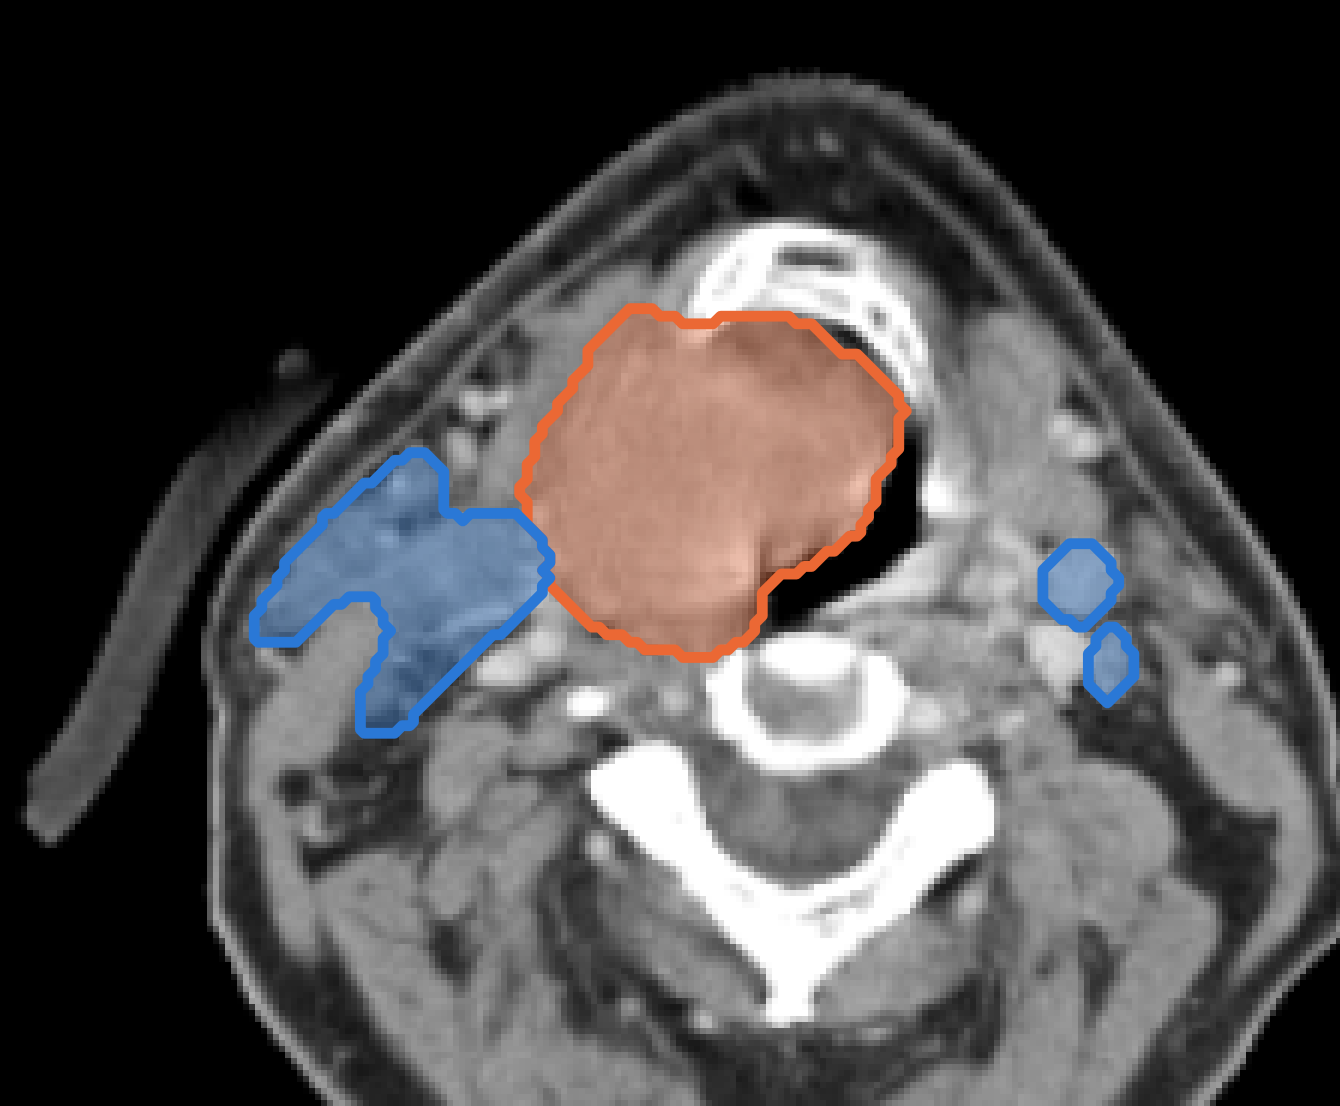
\includegraphics[width=3.1cm]{figures/ct_crop_hn1.png}};
\node[anchor=north, align=center] at (2.30,6.02) {%
  \tikz{\fill[orange!80!red, draw=orange!50!black] (0,0) rectangle (6pt,6pt);}\ primary GTV\enspace
  \tikz{\fill[blue!55!cyan, draw=blue!50!black] (0,0) rectangle (6pt,6pt);}\ nodal GTV\\[1pt]
  \textbf{whole tumour = primary $\cup$ nodal}};
\draw[arr] (2.30,5.28) -- (2.30,5.05);
% feature bar (widths proportional to 14 / 93 / 372 of 479 features)
\node[font=\sffamily\fontsize{7}{8}\selectfont\bfseries] at (2.30,4.85) {479 radiomic features (PyRadiomics)};
\fill[orange!75!black] (0.40,4.15) rectangle (0.52,4.60);
\fill[orange!55]       (0.52,4.15) rectangle (1.30,4.60);
\fill[orange!25]       (1.30,4.15) rectangle (4.20,4.60);
\draw[orange!50!black] (0.40,4.15) rectangle (4.20,4.60);
\node[lab, anchor=north, align=center] at (2.30,4.08) {%
  \tikz\node[key, fill=orange!75!black]{};\ shape 14\enspace
  \tikz\node[key, fill=orange!55]{};\ original 93\enspace
  \tikz\node[key, fill=orange!25]{};\ LoG-filtered 372};
\draw[arr] (2.30,3.68) -- (2.30,3.45);
% selection funnel
\filldraw[fill=orange!18, draw=orange!55!black, rounded corners=2pt] (0.30,3.42) -- (4.30,3.42) -- (3.50,2.42) -- (1.10,2.42) -- cycle;
\node[align=center, text width=3.4cm] at (2.30,2.95) {\textbf{Feature selection}\\mRMR, LASSO or filter\\on training data only};
\draw[arr] (2.30,2.42) -- (2.30,2.10);
% node feature vector
\foreach \i in {0,...,3} \node[cell, fill=orange!65] at (1.05+0.42*\i,1.82) {};
\foreach \i in {0,...,2} \node[cell, fill=green!55!black!70] at (2.85+0.42*\i,1.82) {};
\node[anchor=east, font=\sffamily\fontsize{8}{9}\selectfont\bfseries] at (0.80,1.82) {$\mathbf{x}_i$};
\node[lab, anchor=north, align=center] at (1.68,1.52) {2, 4 or 8\\radiomic};
\node[lab, anchor=north, align=center] at (3.27,1.52) {T, N, volume\\(optional)};
\node[anchor=south, align=center, text=orange!40!black] at (2.30,0.12) {\textbf{one feature vector per patient}};

%% ================================================================ 2  patient-similarity graph
\begin{scope}[shift={(5.15,4.15)}]
  \node[tr0] (p1) at (0.30, 3.40) {};
  \node[tr0] (p2) at (1.25, 3.85) {};
  \node[tr1] (p3) at (2.30, 3.55) {};
  \node[tr0] (p4) at (3.20, 3.95) {};
  \node[tr0] (p5) at (0.55, 2.35) {};
  \node[tr1] (p6) at (1.60, 2.75) {};
  \node[tr0] (p7) at (2.95, 2.70) {};
  \node[tr0] (p8) at (0.25, 1.20) {};
  \node[tr0] (p9) at (2.70, 1.45) {};
  \node[tr1] (p10) at (3.25, 0.70) {};
  \node[tr0] (p11) at (1.00, 0.35) {};
  \node[test] (t1) at (1.60, 1.10) {};
  \begin{scope}[on background layer]
    \foreach \a/\b in {p1/p2, p2/p3, p3/p4, p1/p5, p2/p6, p5/p6, p3/p6, p4/p7, p3/p7, p6/p7, p5/p8, p7/p9, p9/p10, p7/p10, p6/p9, p8/p11, p11/p9}
      \draw[black!28, line width=0.5pt] (\a) -- (\b);
    \foreach \a in {p5, p6, p8, p9}
      \draw[orange!85!black, line width=0.9pt, ->, >={Stealth[length=4pt]}, shorten >=2pt] (\a) -- (t1);
  \end{scope}
\end{scope}
\node[align=left, anchor=north west] at (5.00,4.00) {%
  \tikz\node[tr0]{};\ training patient, no event\\[1.5pt]
  \tikz\node[tr1]{};\ training patient, event\\[1.5pt]
  \tikz\node[test, minimum size=9pt]{};\ test patient (outcome unseen)};
\node[note=blue, text width=3.45cm, anchor=north] at (6.75,2.55) {%
  \textbf{Edges:} each patient receives links from its 5, 10 or 20 most similar \emph{training} patients (cosine similarity of $\mathbf{x}_i$).\\[2pt]
  \textbf{No leakage:} test patients receive links but never send them.};

%% ================================================================ 3  network
\begin{scope}[every node/.append style={}]
\node[blk=blue, text width=9.5mm, minimum width=10.5mm]   (in)  at (9.50,7.00)  {$\mathbf{x}_i$\\dropout\\0.2};
\node[blk=teal, text width=10mm, minimum width=11mm]      (mp1) at (10.85,7.00) {Message\\passing 1\\(32)};
\node[plus]                                               (s1)  at (11.78,7.00) {+};
\node[blk=teal, text width=10mm, minimum width=11mm]      (mp2) at (12.85,7.00) {Message\\passing 2\\(32)};
\node[plus]                                               (s2)  at (13.78,7.00) {+};
\node[blk=violet, text width=8.8mm, minimum width=9.4mm]      (out) at (14.75,7.00) {Linear\\+\\sigmoid};
\end{scope}
\draw[arr] (in) -- (mp1);
\draw[arr] (mp1) -- (s1);
\draw[arr] (s1) -- (mp2);
\draw[arr] (mp2) -- (s2);
\draw[arr] (s2) -- (out);
% linear skip: Linear(x) added to the output of message passing 1
\draw[arr, draw=black!55] (in.north) -- ++(0,0.42) -| node[pos=0.25, above, lab] {linear skip from input} (s1.north);
% residual: output of layer 1 (h1) added to the output of layer 2
\draw[arr, draw=teal!50!black] ($(s1.east)!0.5!(mp2.west)$) -- ++(0,0.72) -| node[pos=0.25, above, lab, text=teal!40!black] {residual} (s2.north);
\node[lab, align=center, text width=5.9cm] at (12.10,6.02) {Message passing: GCN, GraphSAGE or GAT (4 heads $\times$ 8).\\Each layer is followed by ELU and dropout 0.5.};
% inset: inside one message-passing layer
\node[note=teal, minimum width=6.1cm, minimum height=4.55cm, anchor=north west] (inset) at (9.05,5.55) {};
\node[anchor=north west, font=\sffamily\fontsize{7}{8}\selectfont\bfseries, text=teal!40!black] at (9.15,5.50) {Inside one message-passing layer};
\begin{scope}[shift={(10.25,3.35)}]
  \node[circle, fill=blue!65!cyan!80!black, draw=white, minimum size=17pt, inner sep=0pt, text=white, font=\sffamily\fontsize{7.5}{8}\selectfont\bfseries] (ci) at (0,0) {$i$};
  \node[tr0, minimum size=11pt, text=white, font=\sffamily\fontsize{5.5}{6}\selectfont] (j1) at (-0.85,0.90) {$j$};
  \node[tr1, minimum size=11pt, text=white, font=\sffamily\fontsize{5.5}{6}\selectfont] (j2) at (0.85,0.90) {$j$};
  \node[tr0, minimum size=11pt, text=white, font=\sffamily\fontsize{5.5}{6}\selectfont] (j3) at (-0.85,-0.90) {$j$};
  \node[tr0, minimum size=11pt, text=white, font=\sffamily\fontsize{5.5}{6}\selectfont] (j4) at (0.85,-0.90) {$j$};
  \foreach \j in {j1, j2, j3, j4}
    \draw[->, orange!85!black, line width=0.9pt, shorten >=1pt] (\j) -- (ci);
  \draw[->, black!60, line width=0.7pt] (ci.north east) .. controls +(0.5,0.35) and +(0.5,-0.35) .. (ci.south east);
  \node[lab] at (0.88,0) {self};
  \node[lab, align=center, anchor=north] at (0,-1.20) {neighbours $j$ = training\\patients linked to $i$};
\end{scope}
\node[anchor=north west, align=left, text width=3.55cm] at (11.45,4.95) {%
  Each patient's representation is updated from its own features and those of its neighbours:\\[5pt]
  $\mathbf{h}_i' = \mathbf{W}_0\mathbf{h}_i + \textstyle\sum_{j} w_{ij}\mathbf{W}\mathbf{h}_j$\\[5pt]
  $w_{ij}$: degree-normalised (GCN), mean (GraphSAGE) or learned attention (GAT).};
\node[align=center, text width=6.0cm, text=teal!35!black] at (12.10,0.50) {Training: full batch, 150 epochs, Adam (learning rate 0.005), class-weighted cross-entropy};

%% ================================================================ 4  prediction
\node[align=center, text width=2.3cm] at (16.75,8.15) {\textbf{Probability of event}\\for each patient};
\foreach \y/\e/\f/\c in {7.20/LR (2 y)/0.55/red, 6.35/DM (2 y)/0.30/orange, 5.50/OS (4 y)/0.70/violet}{
  \node[anchor=west] at (15.70,\y+0.28) {\e};
  \fill[black!12, rounded corners=1.5pt] (15.75,\y-0.12) rectangle (17.80,\y+0.08);
  \fill[\c!70!black, rounded corners=1.5pt] (15.75,\y-0.12) rectangle ({15.75+2.05*\f},\y+0.08);
}
\node[lab] at (16.78,4.98) {illustrative values};
\node[note=violet, text width=2.0cm, anchor=north, align=center] at (16.75,4.55) {%
  \textbf{Ten-seed ensemble}\\[2pt]
  \tikz{\foreach \k in {0,...,9} \fill[violet!55] (\k*0.17,0) rectangle +(0.13,0.22);}\\[1pt]
  probabilities averaged over seeds 0--9};
\node[note=violet, text width=2.0cm, anchor=north, align=center] at (16.75,2.45) {%
  \textbf{Evaluation}\\[1pt] AUC on the external HN1 cohort, compared with the published CNN};

%% ================================================================ stage arrows
\draw[stage] (4.35,6.70) -- (5.10,6.70);
\draw[stage] (8.45,7.00) -- (in.west);
\draw[stage] (out.east) -- (16.05,7.00);

%% ================================================================ validation design strip
\node[anchor=west, font=\sffamily\fontsize{7.5}{9}\selectfont\bfseries, text=yellow!25!black] at (0.20,-0.48) {Validation design};
\node[note=blue, text width=3.45cm, anchor=north west, fill=blue!8] (dev) at (0.20,-0.75) {%
  \textbf{Development:} HN-PET-CT, \nPatCan{} patients, four Canadian centres. 5-fold CV or cohort split; model chosen on validation AUC.};
\node[note=orange, text width=3.45cm, anchor=north west, fill=orange!10] (tst) at (4.75,-0.75) {%
  \textbf{External test:} HN1, \nPatMAA{} patients, MAASTRO Clinic. Never used for training or model selection.};
\draw[stage, line width=2.5pt] (dev.east) -- (tst.west);

%% ================================================================ no-edge control strip
\node[anchor=west, font=\sffamily\fontsize{7.5}{9}\selectfont\bfseries, text=black!65] at (9.05,-0.48) {No-edge control (MLP)};
\begin{scope}[every node/.append style={minimum height=8mm, text width=9mm, minimum width=10mm}]
  \node[blk=blue]   (cin) at (9.50,-1.60) {$\mathbf{x}_i$};
  \node[blk=gray]   (l1)  at (10.85,-1.60) {Linear 1\\(32)};
  \node[blk=gray]   (l2)  at (12.85,-1.60) {Linear 2\\(32)};
\end{scope}
\node[plus] (cs1) at (11.78,-1.60) {+};
\node[plus] (cs2) at (13.78,-1.60) {+};
\node[blk=violet, minimum height=8mm, text width=8.8mm, minimum width=9.4mm] (co) at (14.75,-1.60) {Linear +\\sigmoid};
\draw[arr] (cin) -- (l1); \draw[arr] (l1) -- (cs1); \draw[arr] (cs1) -- (l2); \draw[arr] (l2) -- (cs2); \draw[arr] (cs2) -- (co);
\draw[arr, draw=black!55] (cin.north) -- ++(0,0.25) -| (cs1.north);
\draw[arr, draw=teal!50!black] ($(cs1.east)!0.5!(l2.west)$) -- ++(0,0.65) -| (cs2.north);
\node[anchor=west, align=left, text width=2.45cm] at (15.30,-1.50) {Identical network with linear layers in place of message passing, so the graph is ignored. Comparing the two shows what the graph adds.};
\end{tikzpicture}
